\part{Element Buffer}
\frame{\partpage}

\begin{frame}{Creating \& Using Element Buffer}
	\begin{center}
		Live Coding
	\end{center}
\end{frame}

\begin{frame}{Exercise 1 - Let's draw a square!}
\begin{center}
	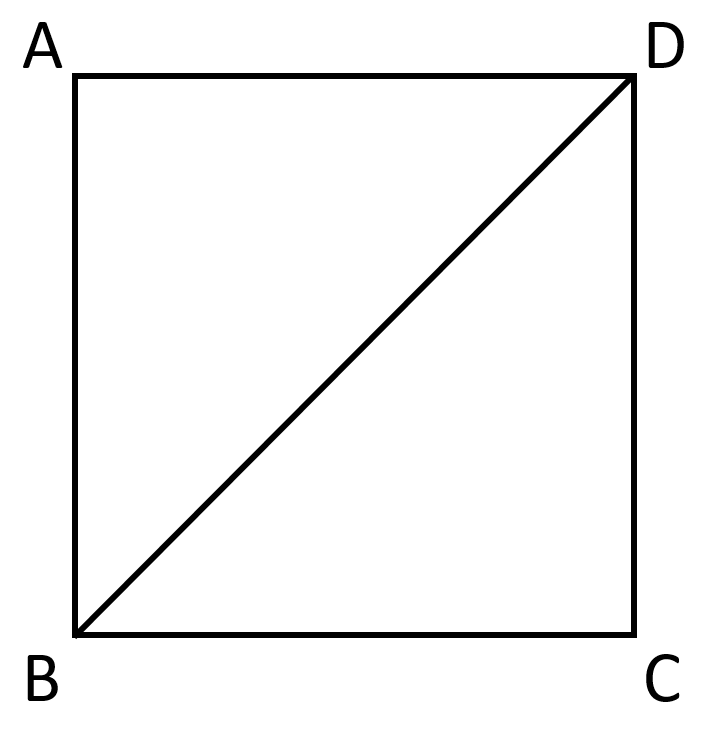
\includegraphics[height=0.8\textheight]{square_vertices}
\end{center}
\end{frame}

\begin{frame}{Exercise 2 - Let's draw a cube!}
	\begin{center}
	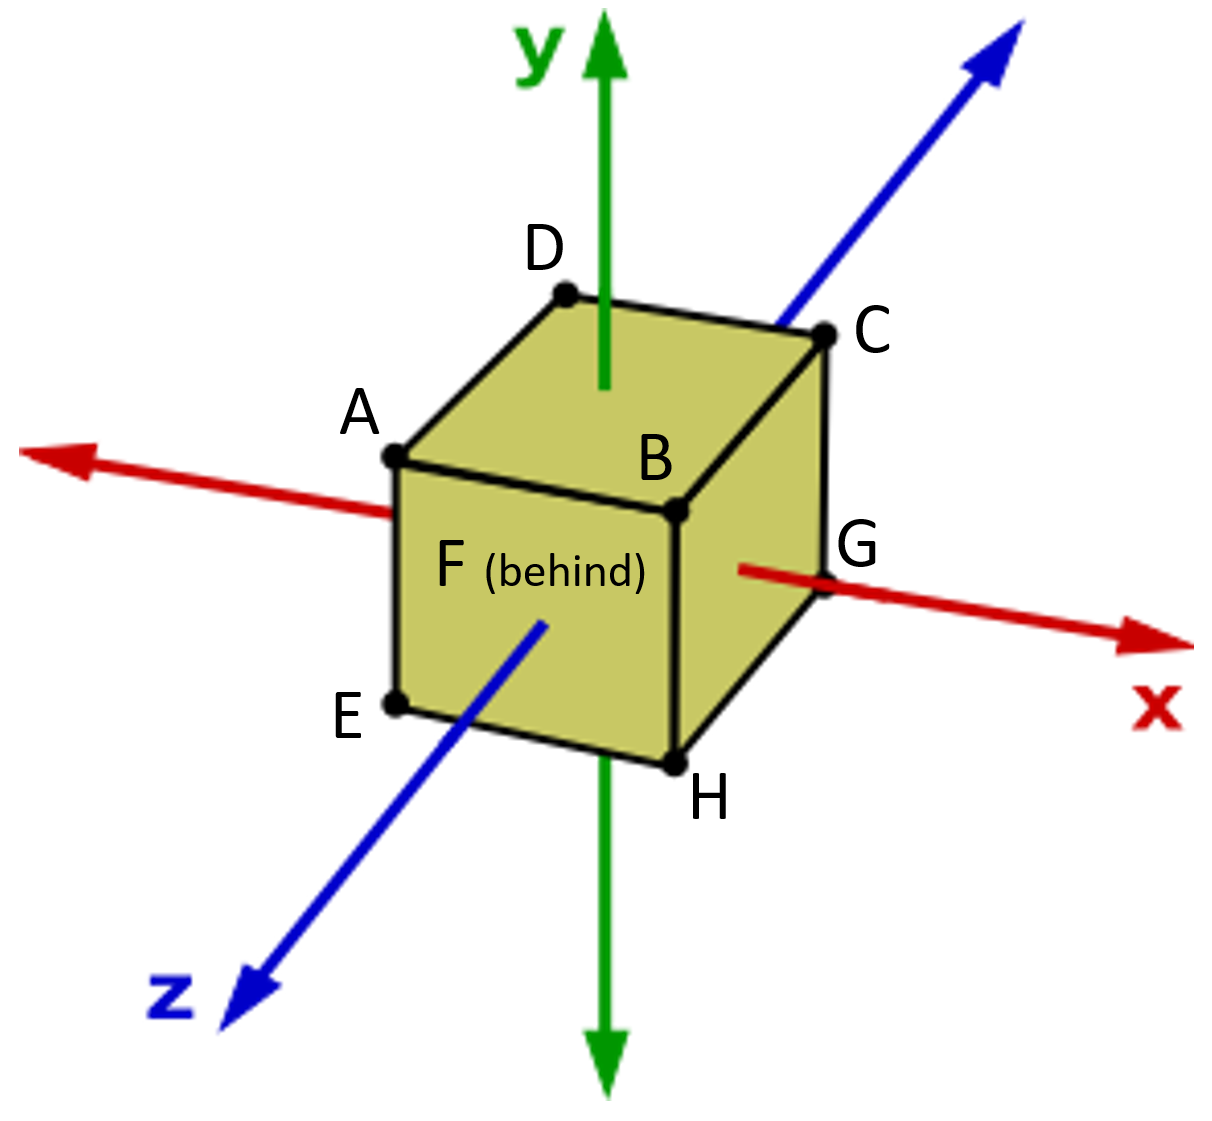
\includegraphics[height=0.8\textheight]{cube_vertices}
	\end{center}
\end{frame}

\begin{frame}{Exercise 3 - Element Buffer}
	\begin{itemize}
		\item Create a cube using an Element Buffer
		\item Create a function which fills a Vertex Buffer and Element Buffer for drawing a Sphere
	\end{itemize}
\end{frame}


